%!TEX program = xelatex
\documentclass[cn,normal,11pt]{../elegantnote}

\usepackage{tikz}
\usetikzlibrary{intersections,quotes,angles}

\title{TikZ \& PGF 学习笔记}

\author{\href{https://github.com/lightjameslyy/}{刘涛}}
\institute{中科院计算所}
\version{0.1}
\date{\today}


\begin{document}
\maketitle

\setlist[itemize]{label=$\circ$}

\begin{enumerate}
    \item straight path。有两种格式:

    \tikz \draw[thick, rounded corners=8pt]
        (0,0) -- (0,2) -- (1,3.25) -- (2,2) -- (2,0) -- (0,2) -- (2,2) -- (0,0) -- (2,0);
    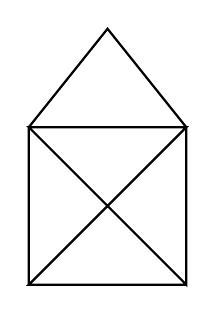
\begin{tikzpicture}
        \draw[thick]
        (0,0) -- (0,2) -- (1,3.25) -- (2,2) -- (2,0) -- (0,2) -- (2,2) -- (0,0) -- (2,0);
    \end{tikzpicture}

    \item curved path:有 1 到 2 个 control 点。比如曲线的起止点是 x 和 y,control 点是 z 和 w。那么在 x 点,曲线的斜率正好是 x 到 z,在 y 点是 w 到 y。

    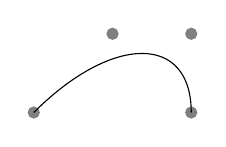
\begin{tikzpicture}
        \filldraw [gray] 
            (0,0) circle [radius=2pt]
            (1,1) circle [radius=2pt]
            (2,1) circle [radius=2pt]
            (2,0) circle [radius=2pt];
        \draw (0,0) .. controls (1,1) and (2,1) .. (2,0);
    \end{tikzpicture}

    \item 用 controls 画一个半圆:
    
    \begin{tikzpicture}
        \filldraw [gray] 
            (-1,0.555) circle [radius=1pt]
            (-0.555,1) circle [radius=1pt]
            (0.555,1) circle [radius=1pt]
            (1,0.555) circle [radius=1pt];
        \draw (-1.5,0) -- (1.5,0);
        \draw (0,-1.5) -- (0,1.5);
        \draw (-1,0) .. controls (-1,0.555) and (-0.555,1) .. (0,1)
            .. controls (0.555,1) and (1,0.555) .. (1,0);
    \end{tikzpicture}

    \item 上面画圆的方法有点复杂,可以直接用 circle 或 ellipse 路径:
    
    \tikz \draw (0,0) circle [radius=10pt];
    \tikz \draw (0,0) ellipse [x radius=20pt, y radius=10pt];

    \item 一个更直观的画圆的方法:
    
    \begin{tikzpicture}
        \draw (-1.5,0) -- (1.5,0);
        \draw (0,-1.5) -- (0,1.5);
        \draw (0,0) circle [radius=1cm];
    \end{tikzpicture}

    \item rectangle:

    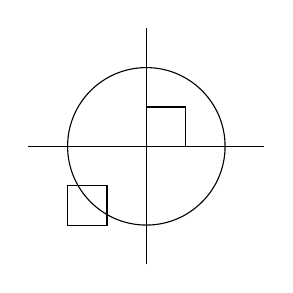
\begin{tikzpicture}
        \draw (-1.5,0) -- (1.5,0);
        \draw (0,-1.5) -- (0,1.5);
        \draw (0,0) circle [radius=1cm];
        \draw (0,0) rectangle (0.5,0.5);
        \draw (-1,-1) rectangle (-0.5,-0.5);
    \end{tikzpicture}

    \item grid:

    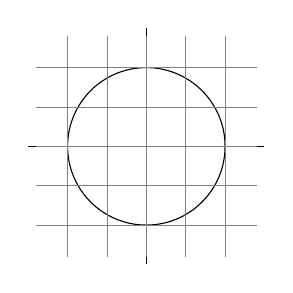
\begin{tikzpicture}
        \draw (-1.5,0) -- (1.5,0);
        \draw (0,-1.5) -- (0,1.5);
        \draw (0,0) circle [radius=1cm];
        \draw[step=.5cm,gray,very thin] (-1.4,-1.4) grid (1.4,1.4);
    \end{tikzpicture}

    \item arc path:
    
    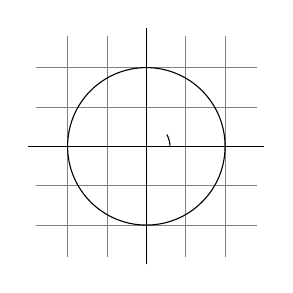
\begin{tikzpicture}
        \draw[step=.5cm,gray,very thin] (-1.4,-1.4) grid (1.4,1.4);
        \draw (-1.5,0) -- (1.5,0);
        \draw (0,-1.5) -- (0,1.5);
        \draw (0,0) circle [radius=1cm];
        \draw (3mm,0mm) arc [start angle=0, end angle=30, radius=3mm];
    \end{tikzpicture}
    \tikz \draw (0,0)
        arc [start angle=0, end angle=315,
        x radius=1.75cm, y radius=1cm];

    \item 通过设置 scale 实现缩放:
    
    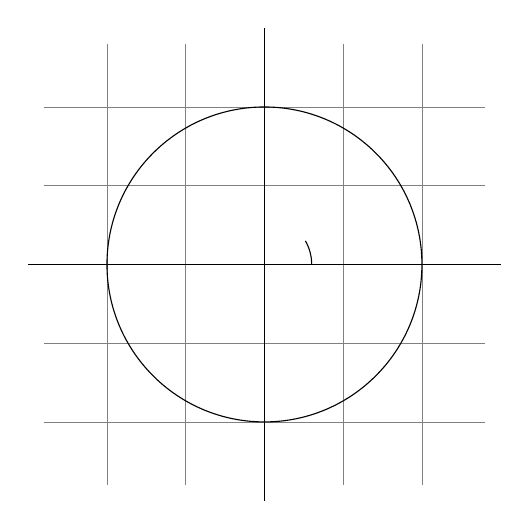
\begin{tikzpicture}[scale=2]
        \draw[step=.5cm,gray,very thin] (-1.4,-1.4) grid (1.4,1.4);
        \draw (-1.5,0) -- (1.5,0);
        \draw (0,-1.5) -- (0,1.5);
        \draw (0,0) circle [radius=1cm];
        \draw (3mm,0mm) arc [start angle=0, end angle=30, radius=3mm];
    \end{tikzpicture}

    \item 使用 clip 截取图的一部分:视窗可以是矩形、圆形……。第一种没有边框,第二种有边框。
    
    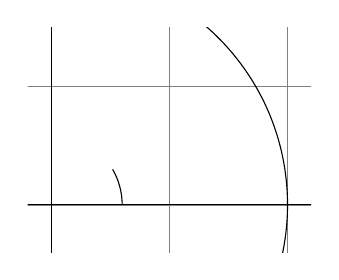
\begin{tikzpicture}[scale=3]
        \clip (-0.1,-0.2) rectangle (1.1,0.75);
        \draw[step=.5cm,gray,very thin] (-1.4,-1.4) grid (1.4,1.4);
        \draw (-1.5,0) -- (1.5,0);
        \draw (0,-1.5) -- (0,1.5);
        \draw (0,0) circle [radius=1cm];
        \draw (3mm,0mm) arc [start angle=0, end angle=30, radius=3mm];
    \end{tikzpicture}
    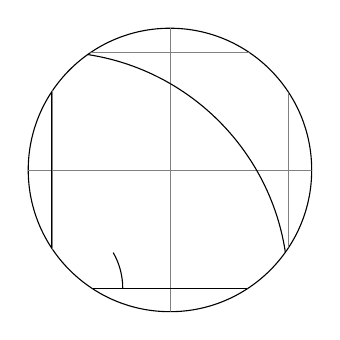
\begin{tikzpicture}[scale=3]
        \clip[draw] (0.5,0.5) circle (.6cm);
        \draw[step=.5cm,gray,very thin] (-1.4,-1.4) grid (1.4,1.4);
        \draw (-1.5,0) -- (1.5,0);
        \draw (0,-1.5) -- (0,1.5);
        \draw (0,0) circle [radius=1cm];
        \draw (3mm,0mm) arc [start angle=0, end angle=30, radius=3mm];
    \end{tikzpicture}

    \item parabola(抛物线)和正余弦:
    
    \tikz \draw (0,0) rectangle (1,1) (0,0) parabola (1,1);
    \tikz \draw[x=3pt,y=3pt] (0,0) parabola bend (4,16) (6,12);
    \tikz \draw[x=1.57ex,y=1ex] (0,0) sin (1,1) cos (2,0) sin (3,-1) cos (4,0)
        (0,1) cos (1,0) sin (2,-1) cos (3,0) sin (4,1);

    \item fill,draw 和 filldraw:\lstinline{[green!20!white]} 的意思是 20\% 的绿色和 80\% 的白色混合。
    
    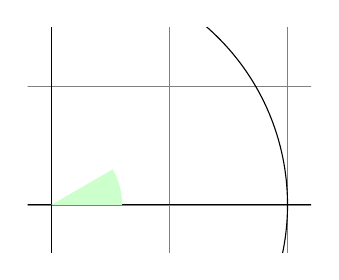
\begin{tikzpicture}[scale=3]
        \clip (-0.1,-0.2) rectangle (1.1,0.75);
        \draw[step=.5cm,gray,very thin] (-1.4,-1.4) grid (1.4,1.4);
        \draw (-1.5,0) -- (1.5,0);
        \draw (0,-1.5) -- (0,1.5);
        \draw (0,0) circle [radius=1cm];
        \fill[green!20!white] (0,0) -- (3mm,0mm)
            arc [start angle=0, end angle=30, radius=3mm] -- (0,0);
    \end{tikzpicture}
    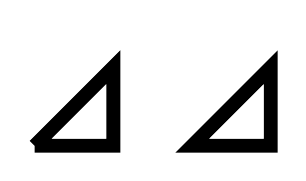
\begin{tikzpicture}[line width=5pt]
        \draw (0,0) -- (1,0) -- (1,1) -- (0,0);
        \draw (2,0) -- (3,0) -- (3,1) -- cycle;
        \useasboundingbox (0,1.5); % make bounding box higher
    \end{tikzpicture}
    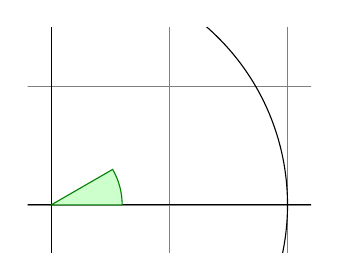
\begin{tikzpicture}[scale=3]
        \clip (-0.1,-0.2) rectangle (1.1,0.75);
        \draw[step=.5cm,gray,very thin] (-1.4,-1.4) grid (1.4,1.4);
        \draw (-1.5,0) -- (1.5,0);
        \draw (0,-1.5) -- (0,1.5);
        \draw (0,0) circle [radius=1cm];
        \filldraw[fill=green!20!white, draw=green!50!black] (0,0) -- (3mm,0mm)
            arc [start angle=0, end angle=30, radius=3mm] -- cycle;
    \end{tikzpicture}

    \item shading:
    
    \tikz \shade (0,0) rectangle (2,1) (3,0.5) circle (.5cm);
    
\begin{tikzpicture}[rounded corners,ultra thick]
        \shade[top color=yellow,bottom color=black] (0,0) rectangle +(2,1);
        \shade[left color=yellow,right color=black] (3,0) rectangle +(2,1);
        \shadedraw[inner color=yellow,outer color=black,draw=yellow] (6,0) rectangle +(2,1);
        \shade[ball color=green] (9,.5) circle (.5cm);
    \end{tikzpicture}

    \item 参考坐标:
    
    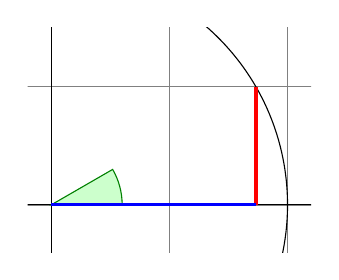
\begin{tikzpicture}[scale=3]
        \clip (-0.1,-0.2) rectangle (1.1,0.75);
        \draw[step=.5cm,gray,very thin] (-1.4,-1.4) grid (1.4,1.4);
        \draw (-1.5,0) -- (1.5,0);
        \draw (0,-1.5) -- (0,1.5);
        \draw (0,0) circle [radius=1cm];
        \filldraw[fill=green!20,draw=green!50!black] (0,0) -- (3mm,0mm)
        arc [start angle=0, end angle=30, radius=3mm] -- cycle;
        \draw[red,very thick] (30:1cm) -- +(0,-0.5);    % 参考坐标是 (30:1cm)
        \draw[blue,very thick] (30:1cm) ++(0,-0.5) -- (0,0);    % 参考坐标是 (30:1cm)+(0,-0.5)
    \end{tikzpicture}

    \item 通过参考坐标定义画 rectangle 的宏:
    
    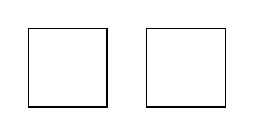
\begin{tikzpicture}
        \def\rectanglepath{-- ++(1cm,0cm) -- ++(0cm,1cm) -- ++(-1cm,0cm) -- cycle}
        \draw (0,0) \rectanglepath;
        \draw (1.5,0) \rectanglepath;
    \end{tikzpicture}
    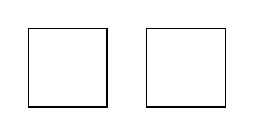
\begin{tikzpicture}
        \def\rectanglepath{-- +(1cm,0cm) -- +(1cm,1cm) -- +(0cm,1cm) -- cycle}
        \draw (0,0) \rectanglepath;
        \draw (1.5,0) \rectanglepath;
    \end{tikzpicture}
    \tikz \draw (0,0) rectangle +(1,1) (1.5,0) rectangle +(1,1);

    \item intersections:求相交。下面的图就是通过两直线相交求 $\tan(30^{\circ})$。
    
    \begin{tikzpicture}[scale=3]
        \clip (-0.1,-0.2) rectangle (1.1,1.51);
        \draw[step=.5cm,gray,very thin] (-1.4,-1.4) grid (1.4,1.4);
        \path [name path=upward line] (1,0) -- (1,1);
        \path [name path=sloped line] (0,0) -- (30:1.5cm); % a bit longer, so that there is an intersection
        % (add ‘\usetikzlibrary{intersections}’ after loading tikz in the preamble)
        \draw [name intersections={of=upward line and sloped line, by=x}]
            [very thick,orange] (1,0) -- (x);
    \end{tikzpicture}

    \item arrows:下面演示给坐标轴加箭头;双向箭头;设置箭头样式。

    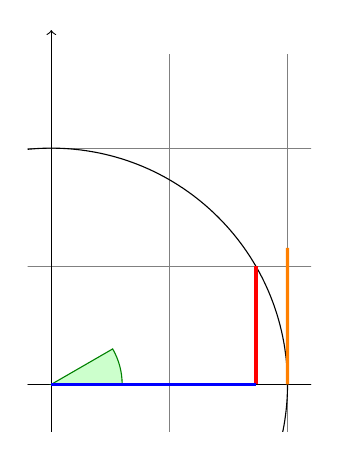
\begin{tikzpicture}[scale=3]
        \clip (-0.1,-0.2) rectangle (1.1,1.51);
        \draw[step=.5cm,gray,very thin] (-1.4,-1.4) grid (1.4,1.4);
        \draw[->] (-1.5,0) -- (1.5,0);
        \draw[->] (0,-1.5) -- (0,1.5);
        \draw (0,0) circle [radius=1cm];
        \filldraw[fill=green!20,draw=green!50!black] (0,0) -- (3mm,0mm)
            arc [start angle=0, end angle=30, radius=3mm] -- cycle;
        \draw[red,very thick] (30:1cm) -- +(0,-0.5);
        \draw[blue,very thick] (30:1cm) ++(0,-0.5) -- (0,0);
        \path [name path=upward line] (1,0) -- (1,1);
        \path [name path=sloped line] (0,0) -- (30:1.5cm);
        \draw [name intersections={of=upward line and sloped line, by=x}]
            [very thick,orange] (1,0) -- (x);
    \end{tikzpicture}
    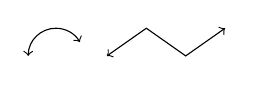
\begin{tikzpicture}
        \draw [<->] (0,0) arc [start angle=180, end angle=30, radius=10pt];
        \draw [<->] (1,0) -- (1.5cm,10pt) -- (2cm,0pt) -- (2.5cm,10pt);
    \end{tikzpicture}
    
\begin{tikzpicture}[>=stealth]
        \draw [->] (0,0) arc [start angle=180, end angle=30, radius=10pt];
        \draw [<<-,very thick] (1,0) -- (1.5cm,10pt) -- (2cm,0pt) -- (2.5cm,10pt);
    \end{tikzpicture}

    \item scoping:制定 scope 内的样式。
    
    \begin{tikzpicture}[ultra thick]
        \draw (0,0) -- (0,1);
        \begin{scope}[thin]
        \draw (1,0) -- (1,1);
        \draw (2,0) -- (2,1);
        \end{scope}
        \draw (3,0) -- (3,1);
    \end{tikzpicture}

    \item transformations:xshift,yshift,shift;rotate;xscale,yscale,scale;xslant,yslant。或者通过 cm 指定转换矩阵。
    
    \tikz \draw (0,0) -- (0,0.5) [xshift=2pt] (0,0) -- (0,0.5);
    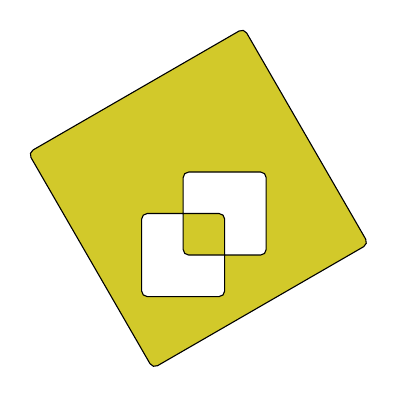
\begin{tikzpicture}[scale=3,even odd rule,rounded corners=2pt,x=10pt,y=10pt]
        \filldraw[fill=yellow!80!black] 
            (0,0) rectangle (1,1)
            [xshift=5pt,yshift=5pt] (0,0) rectangle (1,1)
            [rotate=30] (-1,-1) rectangle (2,2);
    \end{tikzpicture}

    \item for-loops:
    
    \foreach \x in {1,2,3} {$x =\x$, }

    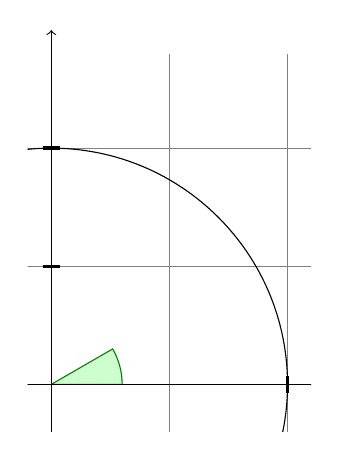
\begin{tikzpicture}[scale=3]
        \clip (-0.1,-0.2) rectangle (1.1,1.51);
        \draw[step=.5cm,gray,very thin] (-1.4,-1.4) grid (1.4,1.4);
        \filldraw[fill=green!20,draw=green!50!black] (0,0) -- (3mm,0mm)
            arc [start angle=0, end angle=30, radius=3mm] -- cycle;
        \draw[->] (-1.5,0) -- (1.5,0);
        \draw[->] (0,-1.5) -- (0,1.5);
        \draw (0,0) circle [radius=1cm];
        \foreach \x in {-1cm,-0.5cm,1cm}
        \draw[very thick] (\x,-1pt) -- (\x,1pt);
        \foreach \y in {-1cm,-0.5cm,0.5cm,1cm}
        \draw[very thick] (-1pt,\y) -- (1pt,\y);
    \end{tikzpicture}

    \tikz \foreach \x in {1,...,10}
        \draw (\x,0) circle (0.4cm);

    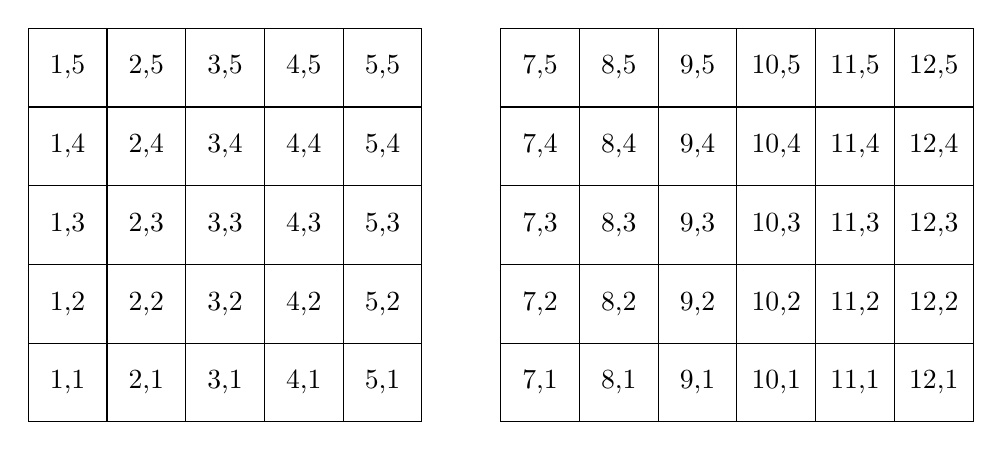
\begin{tikzpicture}
        \foreach \x in {1,2,...,5,7,8,...,12}
            \foreach \y in {1,...,5}
            {
                \draw (\x,\y) +(-.5,-.5) rectangle ++(.5,.5);
                \draw (\x,\y) node{\x,\y};
            }
    \end{tikzpicture}

    \item add text:
    
    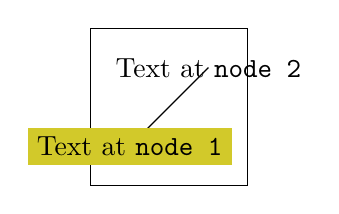
\begin{tikzpicture}
        \draw (0,0) rectangle (2,2);
        \draw (0.5,0.5) node [fill=yellow!80!black]
            {Text at \verb!node 1!}
            -- (1.5,1.5) node {Text at \verb!node 2!};
    \end{tikzpicture}

    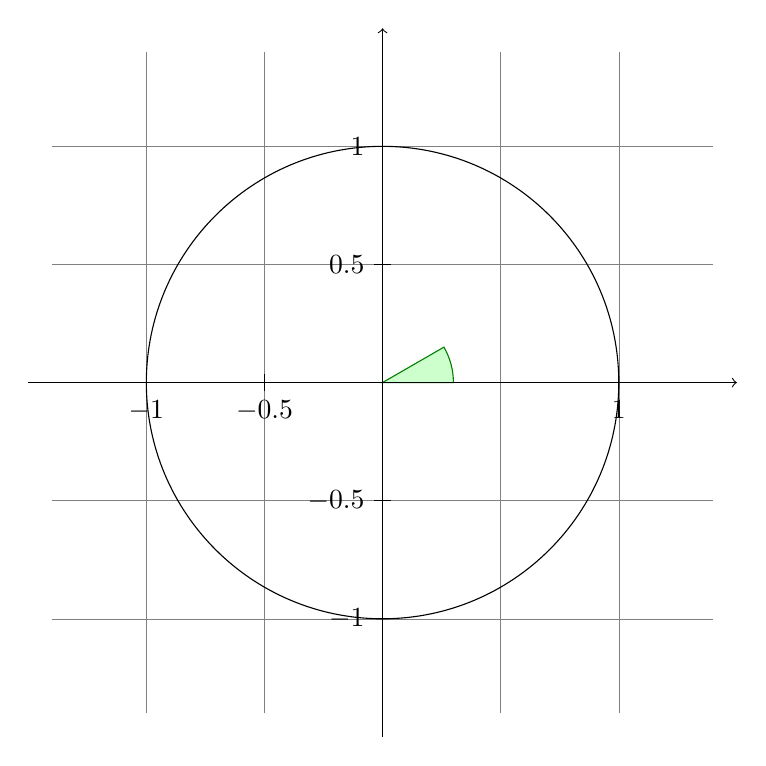
\begin{tikzpicture}[scale=3]
        %\clip (-0.6,-0.2) rectangle (0.6,1.51);
        \draw[step=.5cm,help lines] (-1.4,-1.4) grid (1.4,1.4);
        \filldraw[fill=green!20,draw=green!50!black] (0,0) -- (3mm,0mm)
            arc [start angle=0, end angle=30, radius=3mm] -- cycle;
        \draw[->] (-1.5,0) -- (1.5,0); \draw[->] (0,-1.5) -- (0,1.5);
        \draw (0,0) circle [radius=1cm];
        \foreach \x in {-1,-0.5,1}
            \draw (\x cm,1pt) -- (\x cm,-1pt) node[anchor=north] {$\x$};
        \foreach \y in {-1,-0.5,0.5,1}
            \draw (1pt,\y cm) -- (-1pt,\y cm) node[anchor=east] {$\y$};
    \end{tikzpicture}

    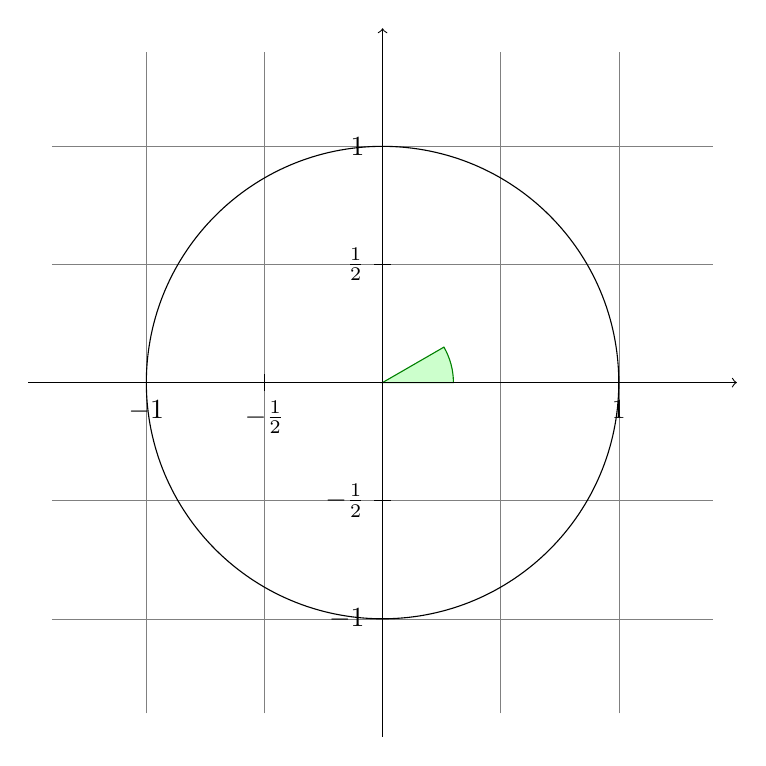
\begin{tikzpicture}[scale=3]
        %\clip (-0.6,-0.2) rectangle (0.6,1.51);
        \draw[step=.5cm,help lines] (-1.4,-1.4) grid (1.4,1.4);
        \filldraw[fill=green!20,draw=green!50!black] (0,0) -- (3mm,0mm)
            arc [start angle=0, end angle=30, radius=3mm] -- cycle;
        \draw[->] (-1.5,0) -- (1.5,0); \draw[->] (0,-1.5) -- (0,1.5);
        \draw (0,0) circle [radius=1cm];
        \foreach \x/\xtext in {-1, -0.5/-\frac{1}{2}, 1}
            \draw (\x cm,1pt) -- (\x cm,-1pt) node[anchor=north] {$\xtext$};
        \foreach \y/\ytext in {-1, -0.5/-\frac{1}{2}, 0.5/\frac{1}{2}, 1}
            \draw (1pt,\y cm) -- (-1pt,\y cm) node[anchor=east] {$\ytext$};
    \end{tikzpicture}

    \item 用 pic 画角:
    
    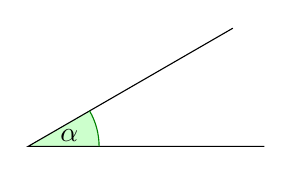
\begin{tikzpicture}[scale=3]
        \coordinate (A) at (1,0);
        \coordinate (B) at (0,0);
        \coordinate (C) at (30:1cm);
        \draw (A) -- (B) -- (C)
            pic [draw=green!50!black, fill=green!20, angle radius=9mm,
                "$\alpha$"] {angle = A--B--C};
    \end{tikzpicture}

    \item 综合:正弦、余弦、正切:

    \begin{tikzpicture}[scale=3]
        % \clip (-2,-0.3) rectangle (2,1.6)
        % 画坐标轴
        \draw[->] (-1.5,0) -- (1.5,0) coordinate (x axis);
        \draw[->] (0,-1.5) -- (0,1.5) coordinate (y axis);
        % 画辅助线
        \draw[step=.5cm,help lines] (-1.4,-1.4) grid (1.4,1.4);
        % 画圆
        \draw (0,0) circle[radius=1cm];
        % 画arc
        \filldraw[fill=green!20!white,draw=green!50!black] (0,0) -- (3mm,0) arc[start angle=0,end angle=30,radius=3mm] -- cycle;
        % sin
        \draw[very thick,red] (30:1cm) -- node[left=1pt,fill=white] {$\sin \alpha$} (30:1cm |- x axis);
        % cos
        \draw[very thick,blue] (0,0) -- node[below=1pt,fill=white] {$\cos \alpha$} (30:1cm |- x axis);
        % tan
        \path[name path=vline] (1,0) -- (1,1);
        \path[name path=sline] (0,0) -- (30:1cm);
        \draw[name intersections={of=vline and sline,by=t}] [very thick,orange]
            (1,0) -- node[right=1pt,fill=white] {$\tan \alpha \color{black}= \frac{\color{red}{\sin \alpha}}{\color{blue}{\cos \alpha}}$} (t);
        \draw (0,0) -- (t);
        % 刻度
        \foreach \x/\xtext in {-1,-0.5/\frac{1}{2},1}
            \draw[thick] (\x cm,1pt) -- (\x cm,-1pt) node[anchor=north,fill=white] {$\xtext$};
        \foreach \y/\ytext in {-1,-0.5/\frac{1}{2},0.5/\frac{1}{2},1}
            \draw[thick] (1pt,\y cm) -- (-1pt,\y cm) node[anchor=east,fill=white] {$\ytext$};
    \end{tikzpicture}

    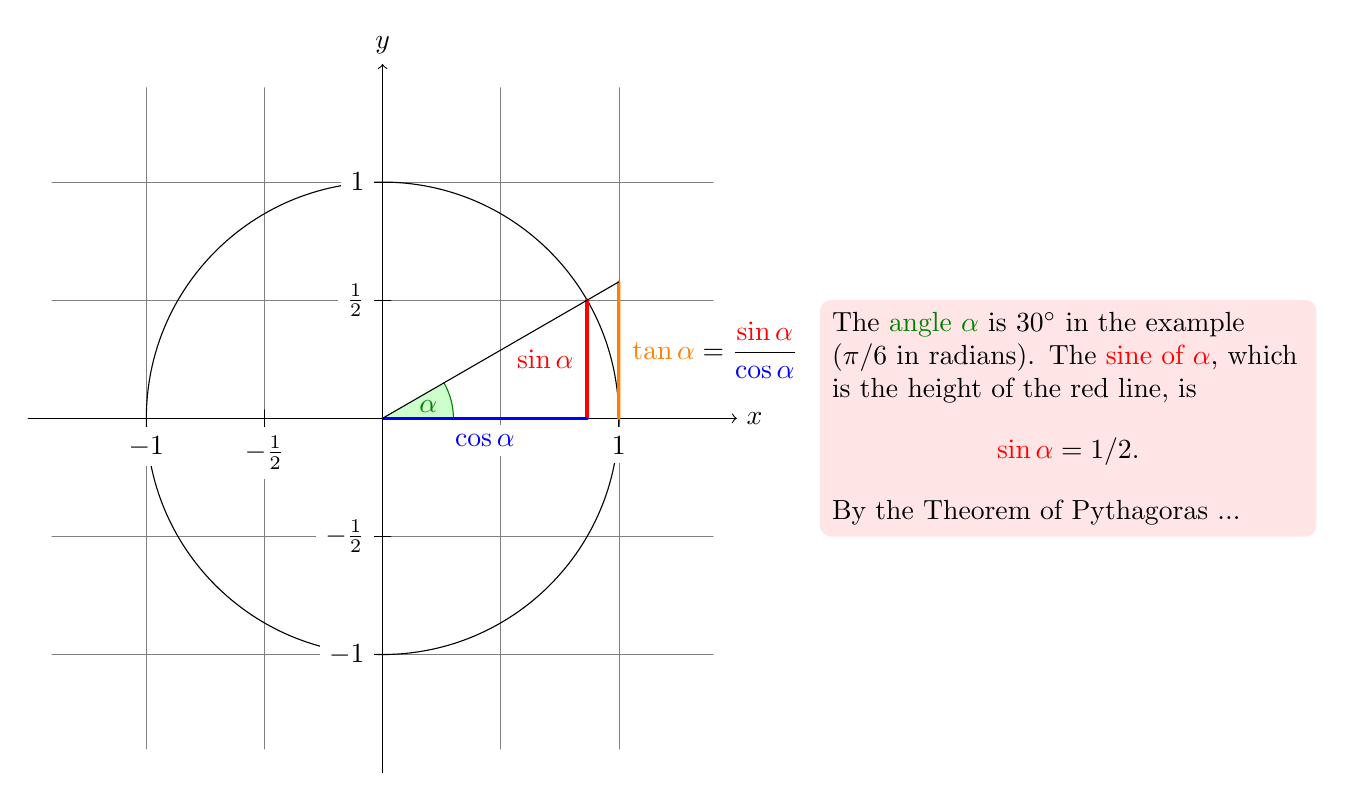
\begin{tikzpicture}
        [scale=3,line cap=round,
        % Styles
        axes/.style=,
        important line/.style={very thick},
        information text/.style={rounded corners,fill=red!10,inner sep=1ex}]
        % Colors
        \colorlet{anglecolor}{green!50!black}
        \colorlet{sincolor}{red}
        \colorlet{tancolor}{orange!80!black}
        \colorlet{coscolor}{blue}
        % The graphic
        \draw[help lines,step=0.5cm] (-1.4,-1.4) grid (1.4,1.4);
        \draw (0,0) circle [radius=1cm];
        \begin{scope}[axes]
        \draw[->] (-1.5,0) -- (1.5,0) node[right] {$x$} coordinate(x axis);
        \draw[->] (0,-1.5) -- (0,1.5) node[above] {$y$} coordinate(y axis);
        \foreach \x/\xtext in {-1, -.5/-\frac{1}{2}, 1}
        \draw[xshift=\x cm] (0pt,1pt) -- (0pt,-1pt) node[below,fill=white] {$\xtext$};
        \foreach \y/\ytext in {-1, -.5/-\frac{1}{2}, .5/\frac{1}{2}, 1}
        \draw[yshift=\y cm] (1pt,0pt) -- (-1pt,0pt) node[left,fill=white] {$\ytext$};
        \end{scope}
        \filldraw[fill=green!20,draw=anglecolor] (0,0) -- (3mm,0pt)
            arc [start angle=0, end angle=30, radius=3mm];
        \draw (15:2mm) node[anglecolor] {$\alpha$};
        \draw[important line,sincolor]
            (30:1cm) -- node[left=1pt,fill=white] {$\sin \alpha$} (30:1cm |- x axis);
        \draw[important line,coscolor]
            (30:1cm |- x axis) -- node[below=2pt,fill=white] {$\cos \alpha$} (0,0);
        \path [name path=upward line] (1,0) -- (1,1);
        \path [name path=sloped line] (0,0) -- (30:1.5cm);
        \draw [name intersections={of=upward line and sloped line, by=t}]
            [very thick,orange] (1,0) -- node [right=1pt,fill=white]
            {$\displaystyle \tan \alpha \color{black}=
            \frac{{\color{red}\sin \alpha}}{\color{blue}\cos \alpha}$} (t);
        \draw (0,0) -- (t);
        \draw[xshift=1.85cm]
            node[right,text width=6cm,information text]
            {
            The {\color{anglecolor} angle $\alpha$} is $30^\circ$ in the
            example ($\pi/6$ in radians). The {\color{sincolor}sine of
            $\alpha$}, which is the height of the red line, is
            \[
            {\color{sincolor} \sin \alpha} = 1/2.
            \]
            By the Theorem of Pythagoras ...
            };
    \end{tikzpicture}

\end{enumerate}


\end{document}
